%%%% Time-stamp: <2012-08-20 17:41:39 vk>

%% example text content
%% scrartcl and scrreprt starts with section, subsection, subsubsection, ...
%% scrbook starts with part (optional), chapter, section, ...
\chapter{Background} \label{cha:background}

In this chapter, we provide preliminary information on the concepts relevant for container orchestration security. These include containers in Section \ref{sec:bkgContainers} and Kubernetes in Section \ref{sec:bkgK8s}.

\section{Containers} \label{sec:bkgContainers}

The aim of containerisation is to provide applications with their own isolated runtime environments and simplify deployment processes. Containers package all code and dependencies an application needs to run and can then be independently run in various computing environments. Thereby, containers address many of the use cases previously tackled by \acp{VM}. 

The main differences between containers and \acp{VM}, as explained by~\textcite{containersVsVMs} and\textcite{containersVsVMsComparison}, are that when using containers, the guest OS is not virtualised on top of a hypervisor, but rather the containers run directly on the host OS using a container daemon. On the one hand, this means that the guests are not fully isolated anymore, as they are using the same host OS. This, on the other hand, comes with significant performance and resource benefits, which is why containers are widely replacing \acp{VM} in many use cases, as found by~\textcite{redhatOutlook}.

In this thesis, we will be primarily looking at Docker\footnote{\url{https://www.docker.com}, accessed 2019-07-18} as the container engine, yet most principles apply to any container platform.

For containerisation, the application and everything it needs is packaged into an image that is then pushed to a \textit{registry}, such as Docker Hub\footnote{\url{https://hub.docker.com}, accessed 2019-07-18}. Registries can either be private or public and can be running in the cloud or locally. From there, the image can be pulled and executed by, for example, a container orchestration system such as Kubernetes. 

\section{Kubernetes} \label{sec:bkgK8s}

\begin{figure}[H]
\begin{center}
    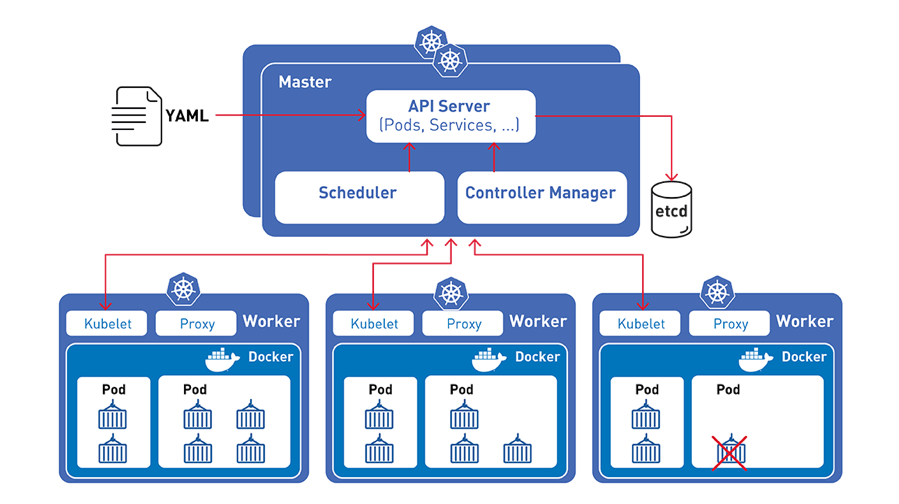
\includegraphics[width=0.8\linewidth]{figures/k8s_architecture.png}
    \caption[Kubernetes Architecture]{This diagram from~\textcite{k8sDiagram} shows the structure of a Kubernetes cluster.}
    \label{fig:k8sArchitecture}
\end{center}
\end{figure}


Kubernetes is a highly flexible and configurable system for container orchestration that provides automatic deployment, scaling, and administration of container applications, as explained in the \textcite{k8sdocs}. 

\paragraph{Architecture}

The Kubernetes architecture is depicted in Figure \ref{fig:k8sArchitecture}. It shows a \textit{cluster}, which is a set of \textit{nodes}\footnote{\url{https://kubernetes.io/docs/concepts/architecture/nodes/}, accessed 2019-07-19} that run the container applications and are displayed as blue boxes in the diagram. Nodes can either be physical or virtual machines, the latter being especially prevalent in hosted public cloud scenarios. Every cluster consists of at least one master and one worker node. 

The master nodes run so-called \textit{control plane components} that are necessary for the cluster to function. These include the \textit{API server} and \mycode{etcd}. The \textit{API server} exposes the \textit{Kubernetes API}\footnote{\url{https://kubernetes.io/docs/concepts/overview/kubernetes-api/}, accessed 2019-07-19}, which is used to control the cluster state. Administrators typically interact with the API using the CLI tool \mycode{kubectl}\footnote{\url{https://kubernetes.io/docs/reference/kubectl/overview/}, accessed 2019-07-19}. The central key-value database \mycode{etcd}\footnote{\url{https://etcd.io}, accessed 2019-07-25} stores all cluster information including all Kubernetes objects and is only supposed to be accessed directly by the API server. The nodes are provided with the necessary information via the API server and \mycode{etcd}.

Worker nodes run the container daemon and the \textit{kubelet}, which is an agent responsible for managing the node. On the workers, the actual containerised applications run. The containers reside within \textit{pods}\footnote{\url{https://kubernetes.io/docs/concepts/workloads/pods/pod/}, accessed 2019-07-19}. A pod runs one or more containers on the same node. Pods are the smallest units that can be scheduled to run. They, like all other Kubernetes objects, are declaratively specified in the \textit{YAML} format\footnote{\url{https://yaml.org}, accessed 2019-07-19}. These specifications include the URL to the container images in the registry, metadata and configuration information. Examples of specification files are given throughout this thesis and in Appendix \hyperref[apx:A]{A}. To create a pod, its specification is submitted to the Kubernetes API. The control plane takes care of the deployment and scheduling of the specified pod. To do so, first, the \textit{Controller manager} determines the demand for pods, then, the \textit{Scheduler} finds a node on which they should run. Finally, the \mycode{kubelet} agent on the node retrieves the configurations from the API server and starts the pod. 

\paragraph{Scaling}

The power of Kubernetes lies in its more advanced concepts, including \textit{Deployments}\footnote{\url{https://kubernetes.io/docs/concepts/workloads/controllers/deployment/}, \\ accessed 2019-07-19} and \textit{ReplicaSets}\footnote{\url{https://kubernetes.io/docs/concepts/workloads/controllers/replicaset/}, \\ accessed 2019-07-19}. These can be used to define how multiple instances of pods should be run. Kubernetes then takes care that the cluster is always in the desired state, updates are rolled out, and new replicas are spun up if required.

\paragraph{Configuration and Secrets Management}

For configuration and credentials management, Kubernetes provides the objects \textit{ConfigMap} and \textit{Secret}\footnote{\url{https://kubectl.docs.kubernetes.io/pages/app_management/secrets_and_configmaps.html}, accessed 2019-07-18}, which can be configured using YAML specifications. They are then mounted into the containers' file systems or passed along using environment variables so that applications can retrieve them.

\paragraph{Exposing applications}

To expose applications running on a set of pods, \textit{Services}\footnote{\url{https://kubernetes.io/docs/concepts/services-networking/service/}, accessed 2019-07-18} can be used. They can either be employed for internal communication within the cluster or can be bound to an \textit{Ingress}\footnote{\url{https://kubernetes.io/docs/concepts/services-networking/ingress/}, accessed 2019-07-19} to expose them to the public internet. 

%% vim:foldmethod=expr
%% vim:fde=getline(v\:lnum)=~'^%%%%\ .\\+'?'>1'\:'='
%%% Local Variables: 
%%% mode: latex
%%% mode: auto-fill
%%% mode: flyspell
%%% eval: (ispell-change-dictionary "en_US")
%%% TeX-master: "main"
%%% End: 
